\chapter{Testing suite for advection}
\label{chap:testing}

In the development of a model, benchmark tests are paramount to ensure the
accuracy and to check the behaviour of the scheme in real-life configurations.
For transport schemes, idealized test cases are used in practice.  Each test
aims at examining the ability of the scheme to meet one or more of the
properties presented in Section~\ref{sec:properties}. For that, results of
the schemes are compared to the algebraic solution of the test case using error
norms. The tests should be representative of atmospheric situations. In
particular, they should examine the behaviour of a single tracer, as well as the
preservation of the relations between multiple tracers, an important feature for
long-lived atmospheric species. 
Another important aspect of testing a model is to be able to compare it to other
models. This can help judging if its performances are worth the implementation
cost when compared to other state-of-the-art schemes. Unfortunately, there is no
standard testing suite for transport schemes, which makes comparisons difficult.
\cite{Williamson1992} proposed a testing suite in the case of shallow-water
equations. It is a non-divergent and non-deformational test where the algebraic
solution is known at all times.  \cite{Nair2002} and~\cite{Nair2008} presented
deformational test cases with an algebraic solution known only at $t=0$ and after a
full period. Recently, \cite{Lauritzen2012} proposed a test-suite for transport schemes
and a comparison with state-of-the-art models was presented in a following
paper (\cite{Lauritzen2014}).

In this chapter, we present the results of advection in Pangolin using idealized
bi-dimensional test cases. Pangolin is tested further in Chapter~\ref{chap:real_case}, where a
chemistry scheme is added and real data is used.  Here, we focus on
global test cases dealing with difficult situations encountered in atmospheric
transport, such as transport across the poles, deformational and non-divergent
flows. In Section~\ref{sec:validation}, we present two tests where the 
algebraic solution is known at any given time. In Section~\ref{sec:comparison},
Pangolin is compared to other existing transport schemes with the testing suite
of~\cite{Lauritzen2012} and the subsequent results of presented by~\cite{Lauritzen2014}.

\section{Model validation}
\label{sec:validation}
As we opted for an operator-splitting approach, the first test in validating the
models was to check zonal and meridional advection. This was done using 1D
test cases, not presented here. These tests allowed us to ensure the cell
neighbours were properly
computed, especially for meridional advection. It also allowed us to check the
advection across the different symmetry axes, especially the Equator.
In this section, we examine the behaviour of Pangolin in two 2D idealized test
cases, where the algebraic solution is known at any given time.  For all tests
presented in this manuscript, we have ensured that the mass is preserved by
comparing the initial air mass to the air mass at the end of the simulation. As
an example, for a full grid, the total air mass is around $2\times 10^{4}$ and
the variation is of the order of $10^{-9}$, so around $10^{-14}\%$.

\subsubsection{Solid body rotation}
This test is commonly used when comparing advection schemes. The winds
in this test case simply advects the initial distribution in such a way that it
corresponds to a rotation around an axis. Winds are given
by~\cite{Williamson1992}:
\begin{align*}
  u &= U_0 (\cos \theta \cos \alpha + \sin \theta \cos \lambda \sin \alpha),\\
  v &= -U_0 \sin \lambda \sin \alpha,
\end{align*}
where $\theta$ and $\lambda$ are the latitude and longitude respectively.
The axis of rotation is defined by $\alpha$, the angle of rotation between the
$z$-axis and the polar axis.  $U_0$ is set here such as a full rotation is 5
days. The initial distribution is defined as a cosine bell:
\begin{align*}
  q(\lambda, \theta) =
  \begin{cases}
    \displaystyle%
   \frac{h_{\text{max}}}{2}%
    \left(1+\cos\left( \frac{\pi r}{R'}\right) \right) \; \text{if} \; r < R',\\
    0 \quad \text{otherwise},
  \end{cases}
\end{align*}
with $R'=R/3$, $h_{\text{max}}=1$ and $R$ the radius of the Earth. $r$ is the great-circle distance
 from the center of the cosine bell noted $(\lambda_0, \theta_0)$ to $(\lambda,\theta)$:
\begin{equation*}
  r(\lambda, \theta)=R \arccos(\sin\theta_0\sin\theta +
  \cos\theta_0\cos(\lambda-\lambda_0)).
\end{equation*}
The center of the cosine bell is set at $(\lambda_0, \theta_0)=(3\pi/2, 0)$.  We
follow the recommendations of~\cite{Williamson1992} and use different rotation
axes: $\alpha=0, \alpha=0.05, \alpha=\frac{\pi}{2}-0.05$ and
$\alpha=\frac{\pi}{2}$. The maximal wind speed is set such as a full rotation at
the Equator takes 12 days. The time-step for Pangolin is set at 16min, leading
to 1080 iterations for a 12-day simulation. The resolution at the Equator is
set to $0.75\times1.13\degre$ (longitude-latitude) so the global CFL is $0.83$
for the axes $\alpha=0$ and $\alpha=0.05$ ($0.80$ for the axes
$\alpha=\frac{\pi}{2}-0.05$ and $\alpha=\frac{\pi}{2}$).

Results are shown on Fig.~\ref{fig:solid_rot}, with the initial distribution and
the results after a full rotation. The global error norms are presented on
Table~\ref{tab:solid_rot}. The first two configurations execute a solid
rotation with an axis close to the North Pole. As the Equator is an axis of
symmetry, the final distribution of the tracer is, as expected, symmetric on
each side of the Equator. It also allows to check that no mass is lost at the
interface between the two hemispheres. \\
The other two configurations advect the tracer distribution over each pole once.
This is an important test as Pangolin has only 3 cells at each pole,
a potential source of loss of accuracy at the poles when compared to
regular latitude-longitude grids. The shape of the distribution after a full rotation
is distorted in the zonal direction and the extrema are much reduced.
\cite{Hourdin2005} used also the transpolar test case on a regular
latitude-longitude grid with Prather's scheme and van Leer's scheme I. The van
Leer scheme showed a deformation in the shape of the distribution in the
meridional direction. This leads us to conclude that the accuracy of the scheme
is the main reason for this deformation and for numerical diffusion.
Furthermore, there is a sensibility to the "tilting" of rotation axis
($\alpha=\frac{\pi}{2}-0.05$, $\alpha=0.05$), which can be seen in the slight
deformation in one direction of the shape of the distribution
($\alpha=\frac{\pi}{2}-0.05$). This observation is confirmed by the error norms
in Table~\ref{tab:solid_rot}.

\begin{figure}
  \centering
  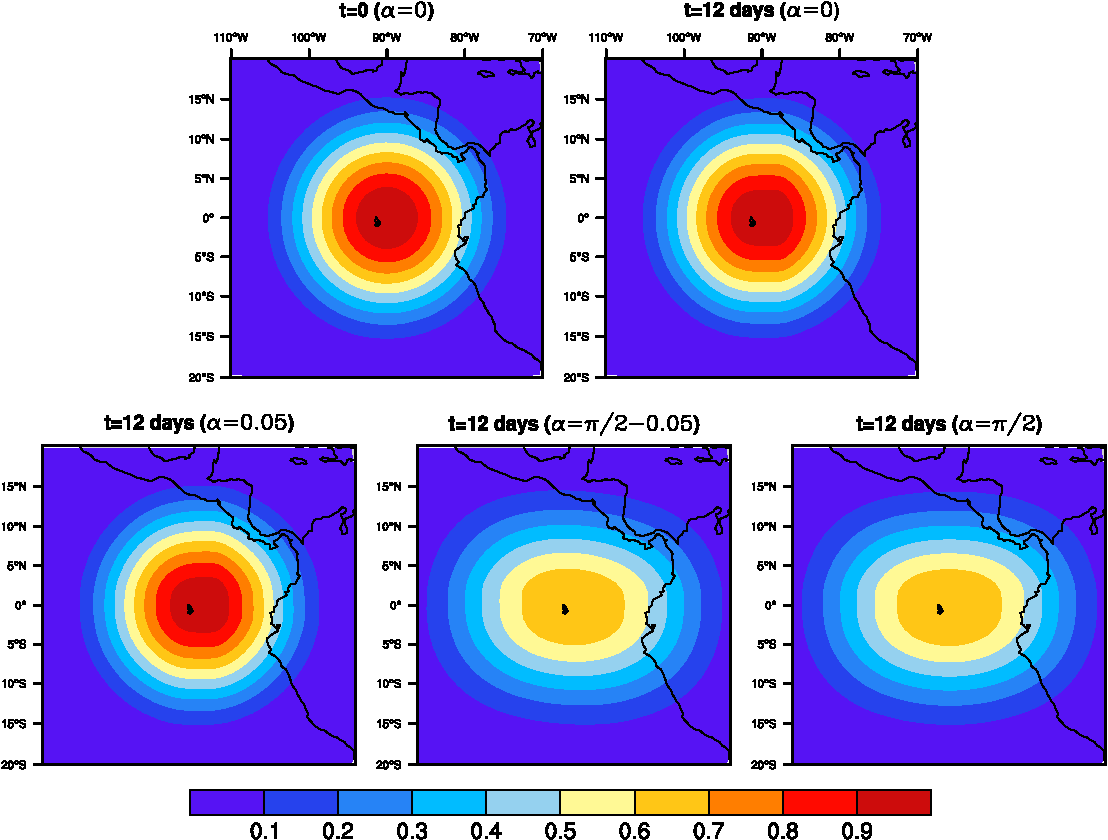
\includegraphics[width=\linewidth]{solid_rot_80lat_all.pdf}
  \caption{Contour plot for the solid body rotation test case at t=0 (upper-left
    figure) and after a full rotation (other figures). The projection used is a
    Lambert conformal projection centered at $(3\frac{\pi}{2}, 0$). The
    resolution at the Equator is $0.75\times1.13\degre$ (longitude and latitude
    respectively). The rotation axis is set at $\alpha=0, \alpha=0.05,
    \alpha=\frac{\pi}{2}-0.05$ and $\alpha=\frac{\pi}{2}$ respectively (from top
    to bottom and left to right).}
  \label{fig:solid_rot}
\end{figure}

\begin{table}
  \centering
  \caption{Error norms for solid rotation, with different rotation axis (defined
    by $\alpha$). The error norms are defined in
    Section~\ref{sec:properties}. The algebraic solution is simply the
  distribution at $t=0$.}
  \label{tab:solid_rot}
  \begin{tabular}{ccc}
    \toprule
    $\alpha$ & $l_2$ & $l_{\infty}$\\
    \midrule 
    0 & 0.0127411765723 & 0.0167418246107 \\
    0.05 & 0.0162542060268 & 0.0274478060601 \\
    $\pi/2-0.05$ & 0.287230024012 & 0.308837928189 \\
    $\pi/2$ & 0.284559486535 & 0.306351598144 \\
    \bottomrule
  \end{tabular}
\end{table}


\subsection{Snail test}
As the previous test did not deform tracer distribution, we examine now the
results using the test presented by \cite{Hourdin1999}.  An initial Gaussian
distribution is deformed by a vortex of winds, thus creating small filaments. As
such, this test can quantify the accuracy of a scheme in preserving these fine
structures. Winds are given by:
\begin{align}
  u =& 2 U_0 \cos{\theta} \sin{\theta} \cos^2 \Big(\frac{\lambda}{2}\Big), \\
  v =& -U_0 \sin{\theta} \cos \Big(\frac{\lambda}{2}\Big) 
  \sin \Big(\frac{\lambda}{2} \Big),
\end{align}
and derive from the following potential:
\begin{equation}
  \Psi = 
  R U_0 \cos^2 \Big(\frac{\lambda}{2}\Big) \cos^2{\theta},
  \label{eqn:potential}
\end{equation}
where $U_0$ is a normalizing speed, $R$ the radius of the Earth.
Winds create a rotation around the axis centered at $(0,0)$ and the period of
rotation depends on the position of the considered point:
\begin{equation*}
  T = \frac{2\pi}{U_0 \cos \theta \cos(\frac{\lambda}{2})}.
\end{equation*}
Here, $U_0$ is chosen such as $T=12$ days at the center $(0, 0)$. For running Pangolin,
the CFL is set at $0.90$ such as a full period takes 384 iterations with a
time-step of $45$ minutes.

The exact solution can be computed algebraically at any time. For that, we use a
Lagrangian approach where the trajectories are the iso-potentials. The initial
position $(\lambda_0, \theta_0)$ of a given point $(\lambda, \theta)$ is found in a
two-step process. First, $\theta_0$ is found by integrating
Eq.~\eqref{eqn:potential}:
\begin{equation*}
  -\alpha \int_0^t \text{sign} \lambda dt = 
  \Bigg[\text{arcsin} 
    \frac{\sin \theta}{\sqrt{1-\frac{\Psi}{R U_0}}} 
    \Bigg]_{\theta_0}^\theta, 
\end{equation*}
with $\alpha=\sqrt{\frac{\Psi U_0}{R^3}}$. Then, $\lambda_0$ is found using the
relation $\Psi(\lambda_0, \theta_0) = \Psi(\lambda, \theta)$.
\begin{figure}
  \subbottom[Initial tracer distribution.]{%
    \includegraphics[width=0.49\linewidth]{{hourdin_160lat_sp_CFL0.9_0}.png}%
    \label{fig:hourdin_0}}
    \hfill
  \subbottom[Simulation after a period.]{%
    \includegraphics[width=0.49\linewidth]{{hourdin_160lat_sp_CFL0.9_T}.png}%
    \label{fig:hourdin_T}}
  \subbottom[Exact solution after a period.]{%
    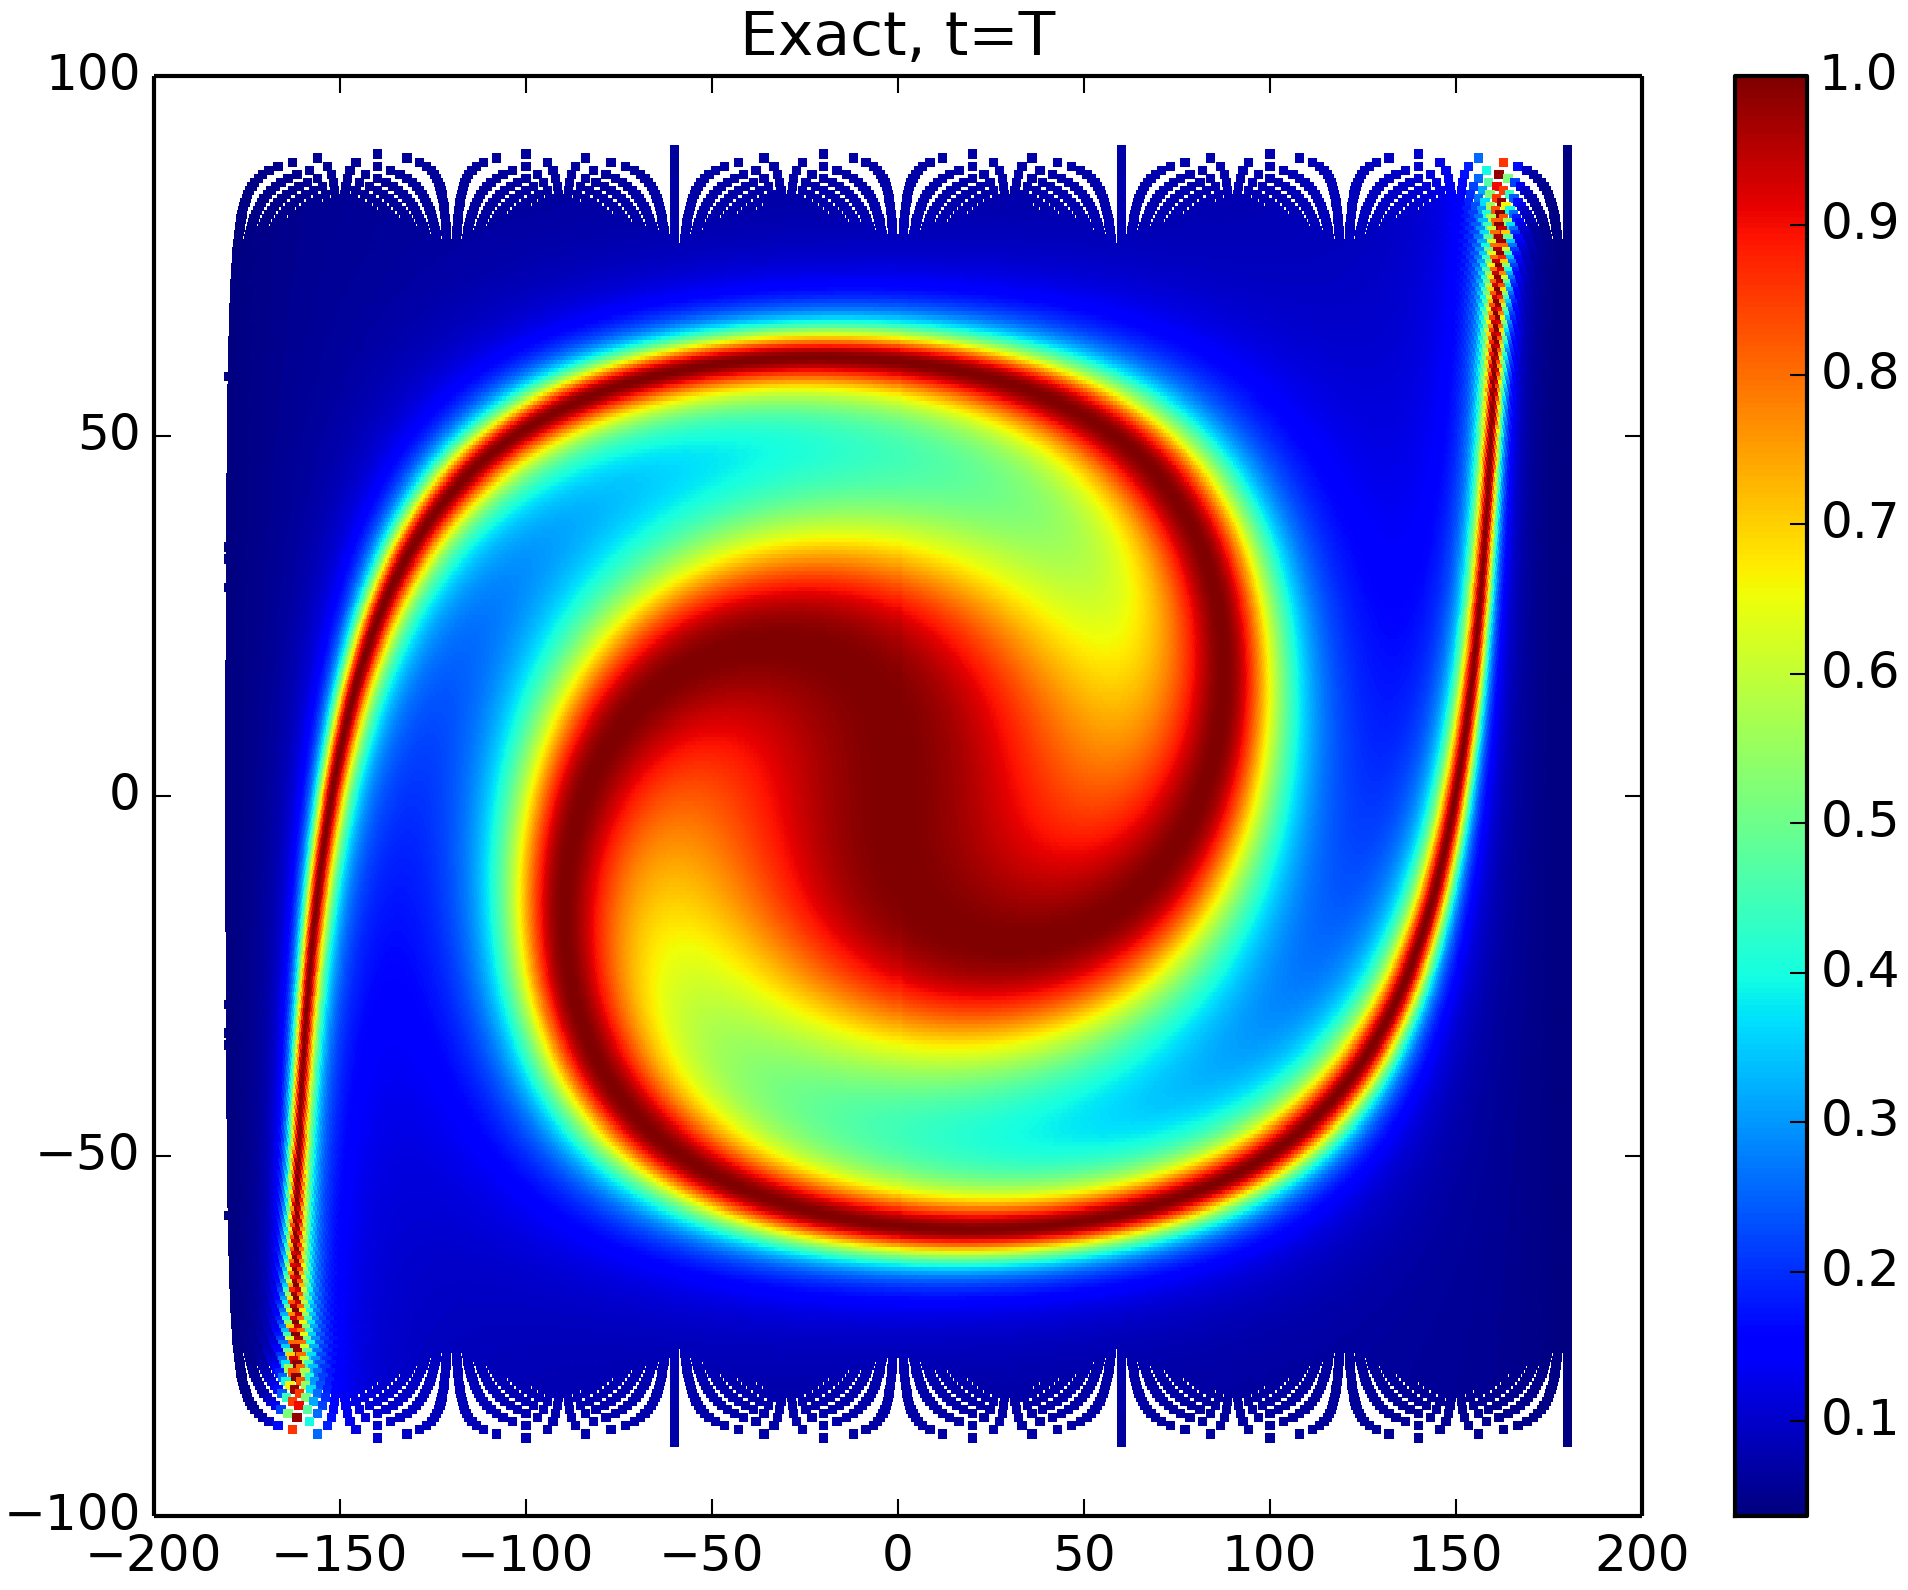
\includegraphics[width=0.49\linewidth]{hourdin_160lat_anal_T.png}%
    \label{fig:hourdin_anal}}
    \hfill
  \subbottom[Relative error after a period.]{%
    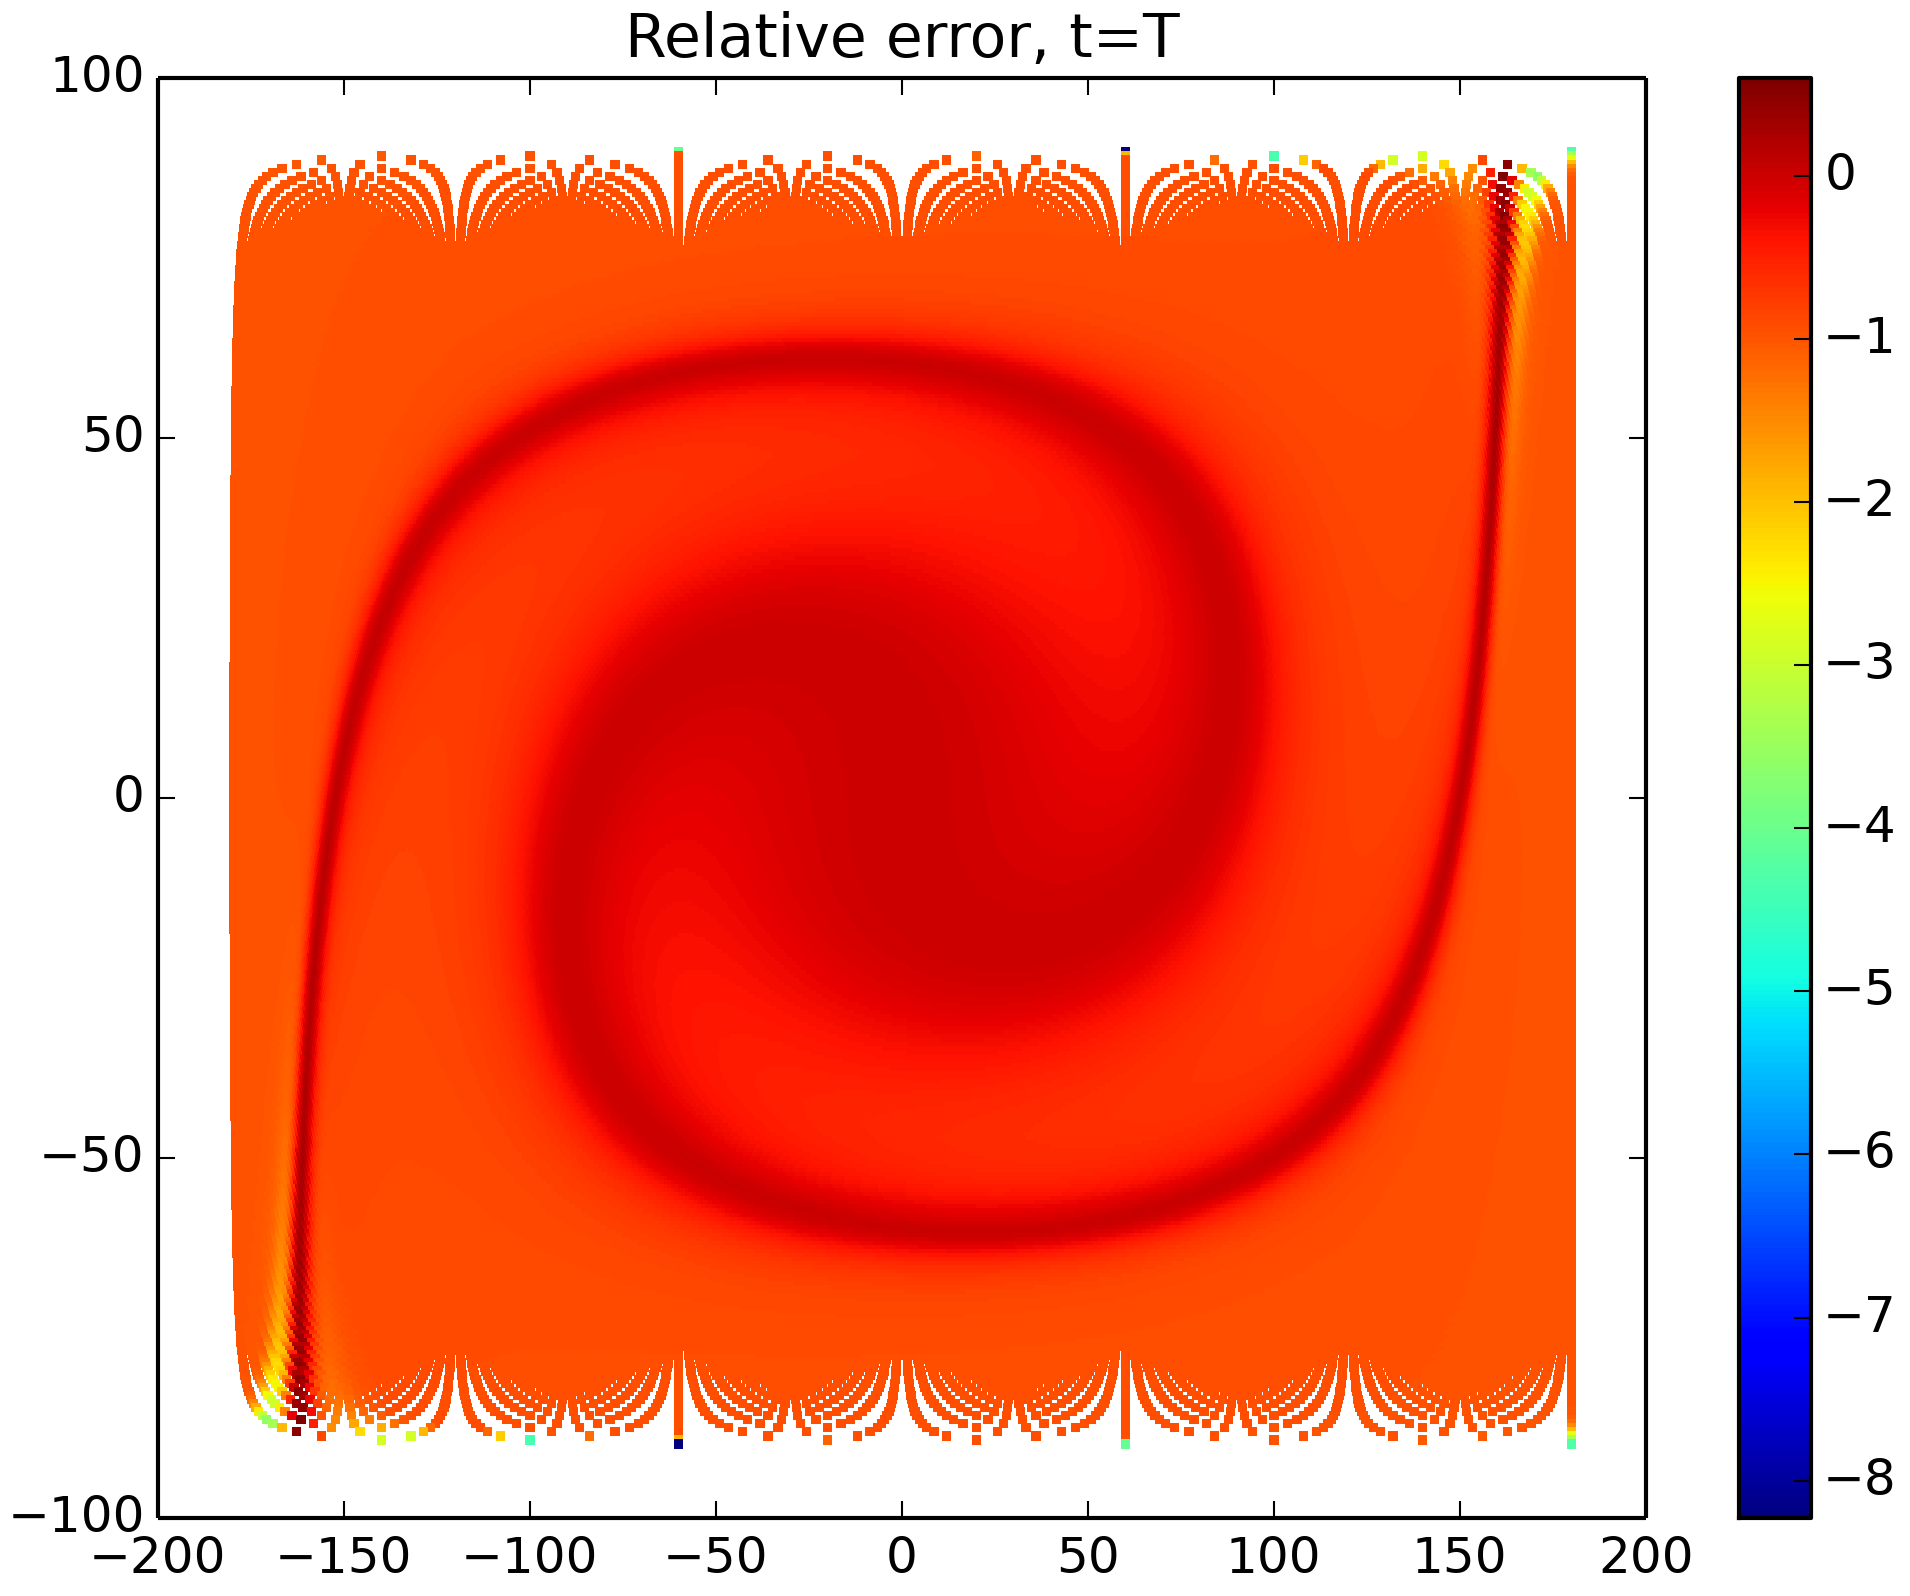
\includegraphics[width=0.49\linewidth]{hourdin_160lat_error_rel_T.png}%
    \label{fig:hourdin_rel}}
  \caption{Tracer distribution at $t=0$ and after a full rotation at the center
    with Hourdin's test case. The data is plotted as scattered points, where each
    point is the center of a cell on the Pangolin grid. No interpolation is done
    and the data is plotted on latitude-longitude coordinates. The grid
    resolution is $0.37\times0.496\degre$ (longitude and latitude respectively).}
\end{figure}

Results are shown on Fig.~\ref{fig:hourdin_T}, while the exact solution given by
the aforementioned method is plotted on Fig.~\ref{fig:hourdin_anal}, along with
the relative error (Fig.~\ref{fig:hourdin_rel}). It can be seen that Pangolin
reproduces faithfully the filaments. Extremas are smoothed due to numerical
diffusion, which is mostly visible near the poles. Most of the error is
localized at the poles, due to numerical diffusion and fewer cells in these
regions.  We also have to ensure there is no local perturbation in the numerical
solution to validate the implementation on the Pangolin grid. For that, we plot
the evolution of two error norms, $l_2$ and $l_{\infty}$,
on~Fig.~\ref{fig:error_hourdin} every 6 hours. As expected, $l_2$ increases
smoothly. Even though a periodic pattern seems to appear in the plot of
$l_{\infty}$, this was not confirmed by further experiments with different
resolutions. However, the global trend of $l_{\infty}$ confirms there is no
numerical artefact in the scheme.
\begin{figure}
  \centering
  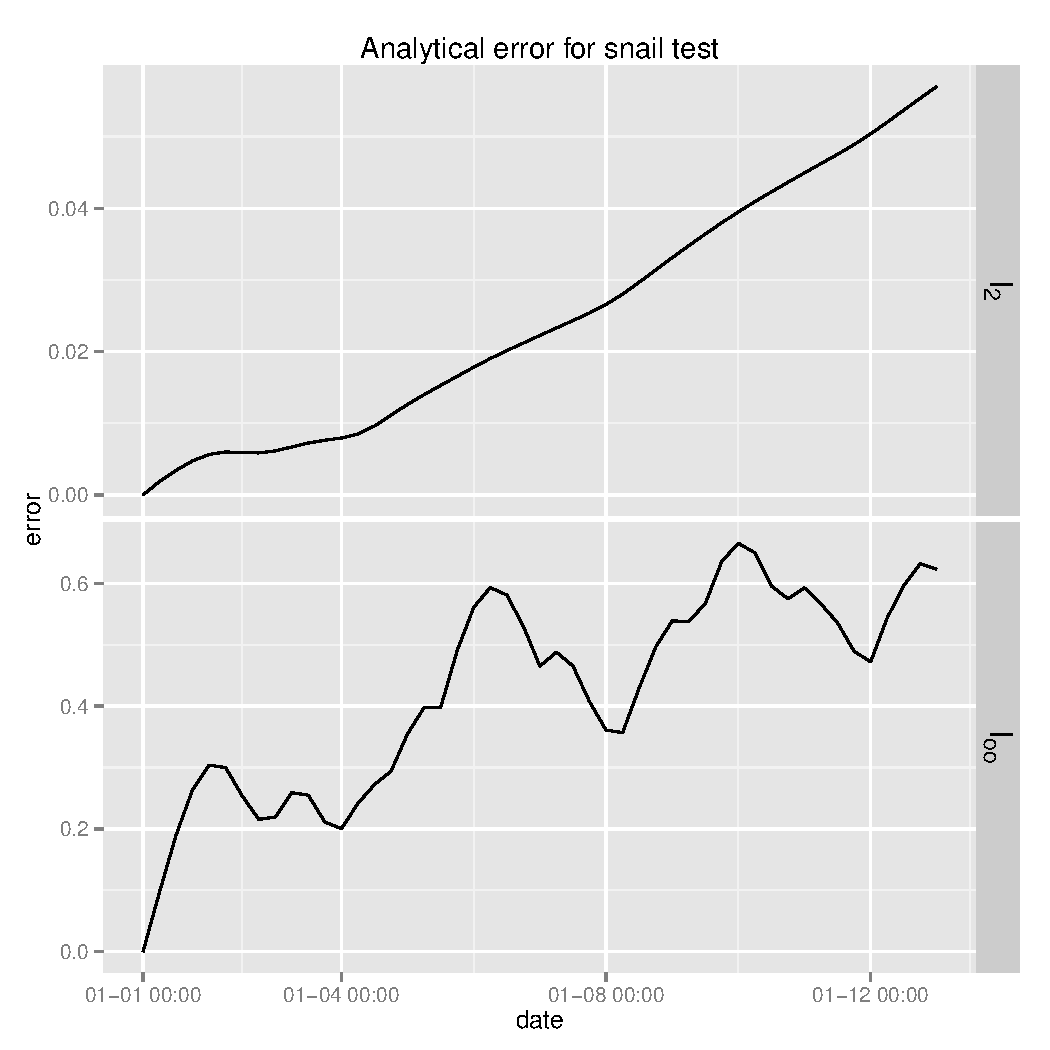
\includegraphics[width=0.7\linewidth]{error_evol_hourdin_80lat.pdf}
  \caption{Evolution of the $l_2$ and $l_{\infty}$ error norms (defined in
  Eq.~\eqref{eqn:err_norms}) for Hourdin's test case during a full rotation (12
  days). The errors are computed every 6 hours. Resolution at the Equator is 
  $0.75\times1.13\degre$ (longitude and latitude respectively).}
  \label{fig:error_hourdin}
\end{figure}

\section{Comparison with other models}
\label{sec:comparison}
As mentioned in the introduction, comparison to other models is paramount for
validating a new transport scheme. A paper was submitted to the \gls{GMD}
journal and is under revision, with a section comparing Pangolin to state-of-the-art schemes. The
comparison is done using the testing suite of~\cite{Lauritzen2012}, with the
results of~\cite{Lauritzen2014}. The full paper is available in
Appendix~\DIFdelbegin \DIFdel{\ref{sec:tests}}\DIFdelend \DIFaddbegin \DIFadd{\ref{sec2:tests}}\DIFaddend , so the reader can refer to it for the
results. Not all tests from the original paper were used in our comparison as we
felt it more relevant to compare Pangolin to schemes with a similar theoretical
order. 

This led us to a selection of five mass-preserving transport models. These 
five schemes were compared to Pangolin with three diagnostics: convergence
rate, preservation of filaments and preservation of preexisting
relations. It should be noted that all the models presented in the tests have a
larger halo than Pangolin: FARSIGHT, CLAW and SLFV-ML use a halo of 2, while
CAM-FV and UCISOM have a halo of 3. This difference can explain the difference
in accuracy between Pangolin, which uses a halo of 1, and other models.
In addition to the tests presented in Appendix~\DIFdelbegin \DIFdel{\ref{sec:tests}}\DIFdelend \DIFaddbegin \DIFadd{\ref{sec2:tests}}\DIFaddend , one more test
of the initial testing suite is presented below.

\subsection{Rough distribution}
The goal of this test is to check how well a scheme suppresses over- and
undershoots using shape-preserving filter. Extrema should be also preserved.
The slotted-cylinder test case is used here to provide a discontinuous initial
distribution defined as:
\begin{equation}
  q(\lambda, \theta) = 
  \begin{cases}
    c \quad \text{if} \; r_i \le r \; \text{and} \; 
    |\lambda-\lambda_i| \ge \frac{r}{6R} \; \text{for} \; i=1,2,\\
    c \quad \text{if} \; r_1 \le r \; \text{and} \; 
    |\lambda-\lambda_1| < \frac{r}{6R} \; \text{and} \; 
    \theta-\theta_1 < \frac{-5r}{12R},\\
    c \quad \text{if} \; r_2 \le r \; \text{and} \; 
    |\lambda-\lambda_2| < \frac{r}{6R} \; \text{and} \; 
    \theta-\theta_2 > \frac{-5r}{12R},\\
    b \quad \text{otherwise},
  \end{cases}
\end{equation}
where $b=0.1$ is the background value and $c=1$ the amplitude. Otherwise, the
notations are the same as in Appendix~\DIFdelbegin \DIFdel{\ref{sec:tests}}\DIFdelend \DIFaddbegin \DIFadd{\ref{sec2:tests}}\DIFaddend .  The impact of a
shape-preserving limiter for Pangolin is shown on Fig.~\ref{fig:slotted} after a
full period. As it can be expected, the diffusion smoothes the maxima and
spreads out the minima. However, it does not completely remove the undershoots
for Pangolin.  Other models are shown at $t=T/2$ on Fig.~\ref{fig:slotted_comp}.
It should be noted FARSIGHT is not present in this comparison as its data were
not available in the original paper. All the other models are given for a fixed
resolution at the Equator of $0.75\degre$. Pangolin does not match this
resolution but is set to match the number of cells of most models, except CLAW.

Without shape-preserving filter, all models show evidence of undershoots as "ripples"
(light blue in the figure) in the background. CLAW and SLFV-ML also show overshooting (red
lines). For Pangolin, CLAW and UCISOM, using a limiter does not
completely remove undershooting. However, \cite{Lauritzen2014} noted the
limiter of UCISOM was relaxed to avoid too much diffusion, thus explaining the
undershooting.
For our selection, CLAW is the only model which does not remove overshooting
with limiters.

\begin{figure}
  \centerline{%
    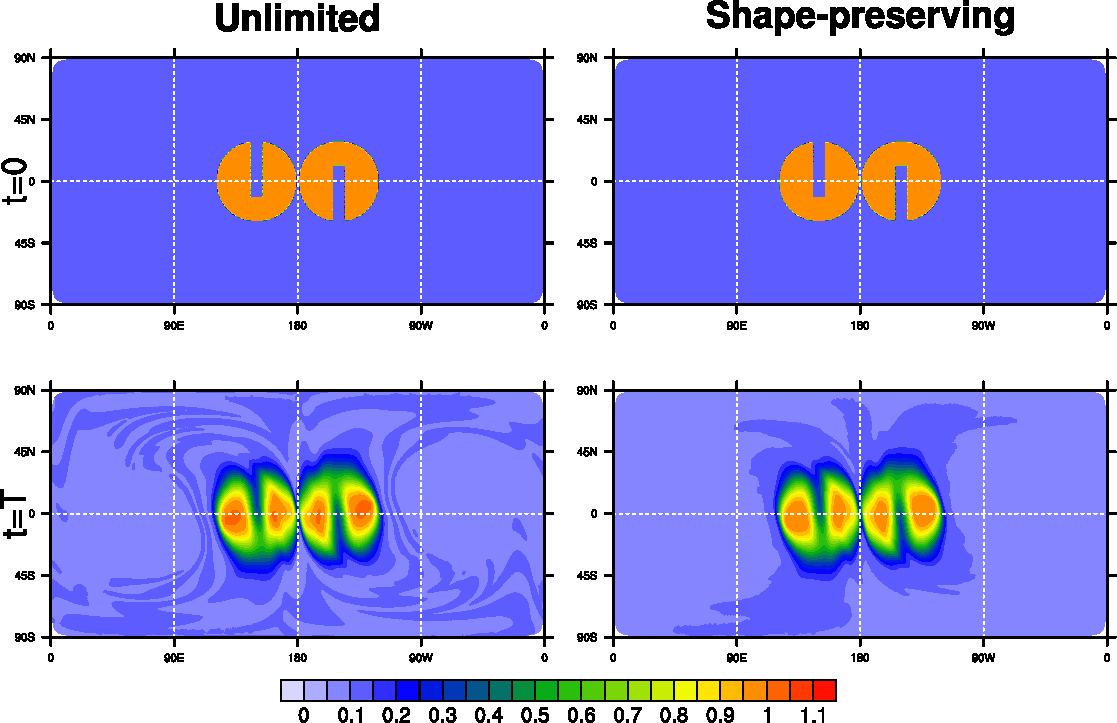
\includegraphics[width=\linewidth]{slotted_cylinders_pango.pdf}%
  }
 \caption{Initial and final concentration for the slotted cylinders test
  case. The model is Pangolin, with $0.56\times0.37\degre$ as resolution on the
  Equator with slope limitation.}
  \label{fig:slotted}
\end{figure}

\begin{figure}
  \centering
  \includegraphics[width=0.8\linewidth]{slotted_cylinders_all.pdf}
  \caption{Tracer concentration for the slotted cylinders case, at $t=T/2$. The
    models are shown with both unlimited and shape-preserving versions of the
    models. All models, except Pangolin which has $0.37\degre$, use a resolution
  of $0.75\degre$ at the Equator. Empty plots correspond to missing data.}
  \label{fig:slotted_comp}
\end{figure}

\section{Conclusion}
The tests presented in this chapter show the performances of Pangolin in regard
to the different properties discussed in Section~\ref{sec:properties} and
compare them to other state-of-the-art advection schemes. Pangolin does compete
with the other models for the preservation of linear relations between two
tracers. However, due to the numerical diffusion of Pangolin, the impact of the slope
limiter on accuracy is found to be small for most of the tests compared to the other
models. Nevertheless, the slope limiter efficiently preserves the shape of the
distribution, as demonstrated in the slotted cylinder test. Like the other
models, Pangolin ensures mass is preserved globally, an important property for
chemistry transport models. 

Pangolin is theoretically second-order accurate and was compared to
schemes with a similar order on diverse grids (see Table~\ref{table:models} for
a summary). It was found the numerical convergence speed of Pangolin is slower than the
theoretical order, possibly due to the linear interpolation done when computing
the meridional gradient. The other schemes presented here achieve a numerical
convergence speed close to two in optimal configurations. However, they use a
larger stencil than Pangolin. Pangolin was designed with a smaller stencil to
reduce communication costs in order to improve scalability. Another measure of
accuracy, the preservation of filaments, confirms that Pangolin can match the
results of the other models, working on non latitude-longitude grids, provided
that a finer grid is used. In conclusion, our strategy is to compensate the loss
of accuracy by using finer resolutions and by exploiting and maintaining good
scalability to run efficient simulations on current supercomputers.
